% \appendix is already called in main.tex

\section{Submodularity of the coverage objective}
\label{app:submodular}

Fix a concept $m \in M$ and consider a random walk $w = (w_0, \dots, w_L)$ on $G_D$ that starts at $w_0 = m$, follows a uniformly chosen outgoing edge at each step, and stops after $D$ steps or at a concept without outgoing edges.
The distribution of $w$ does not depend on $T$, and by acyclicity the walk never visits a concept twice.
Let $\pi_j = \prod_{i=1}^{j} \lambda(w_i)$ be the factor accumulated after $j$ hops, with $\lambda(v) = \lambda$ for every $v$ under the uniform decay of Eq.~\eqref{eq:coverage} (so $\pi_j = \lambda^j$) and $\lambda(v) \in [0, 1]$ under the status-dependent decay of Eq.~\eqref{eq:coverage-status}.
Unrolling the recursion gives
\[
S_D(m, T) = \mathbb{E}_w\big[\, g_w(T) \,\big], \qquad g_w(T) = \max_{j \,:\, w_j \in T} \pi_j ,
\]
with $g_w(T) = 0$ if the walk visits no token.
Since every factor is at most 1, $\pi_j$ never increases with $j$, so the maximum is attained at the first token visited, which is where the recursion stops.
For a fixed walk, $g_w$ assigns to each visited concept a non-negative weight and returns the largest weight among the selected tokens.
Such a maximum of non-negative weights is normalized, monotone and submodular \cite{krause2014submodular}.
These properties are preserved under non-negative linear combinations, hence under the expectation over $w$ and the average over $m \in M$, so $F_D$ is normalized, monotone and submodular for any factors in $[0, 1]$.

\section{Notation and selection algorithms}
\label{app:notation}
\label{app:algorithms}

\begin{table}[h]
\centering
\small
\begin{tabular}{@{}ll@{}}
\toprule
\textbf{Symbol} & \textbf{Meaning} \\
\midrule
$G = (V, E)$, $\mathcal{R}$ & ontology as a DAG with typed edges $E \subseteq V \times \mathcal{R} \times V$; relationship types \\
$d(u, v)$ & hop distance from $u$ to $v$ \\
$M$, $\Mhero$ & concepts to represent: mapped concepts; concepts of the HERO data \\
$r$, $D$ & root concept; hop radius \\
$V_D$, $G_D = (V_D, E_D)$ & candidate pool and the subgraph it induces \\
$\mathrm{Out}(u)$, $\mathrm{In}(u)$, $\deg^+(u)$ & outgoing and incoming edges of $u$ in $G_D$; out-degree \\
$T$, $k$ & token set; token budget $k = |T|$ \\
$\lambda$, $\lambda(v)$ & distance decay; status-dependent factor of a hop into $v$ \\
$h$, $S_h(u, T)$ & horizon; semantic coverage of $u$ by $T$ at horizon $h$ \\
$F_D(T)$ & selection objective, mean of $S_D(m, T)$ over $M$ \\
$\Delta(t \mid T)$ & marginal gain of adding $t$ to $T$ \\
$n_m$, $u_m$, $\ell_i$ & tokens, uncovered branches and token depths in the context tree of $m$ \\
$c_m$, $p_m$, $\mathrm{PC}_m$ & branch coverage, proximity and proximity-coverage score of $m$ \\
$\sigma_m$, $N_s$ & signature of the tree of $m$; number of concepts with signature $s$ \\
\bottomrule
\end{tabular}
\caption{Notation.}
\label{tab:notation}
\end{table}

Algorithm~\ref{alg:select-tokens} gives the lazy greedy selection of Section~\ref{sec:method:selection}, and Algorithm~\ref{alg:candidate-delta} the incremental computation of a marginal gain.
\textsc{CandidateDelta}$(t)$ propagates the change caused by adding $t$ backward along incoming edges, one hop per round, and touches only the concepts that reach $t$ within $D$ hops.
The initial pass makes $|V_D|$ independent calls, which can run in parallel, and builds the heap in $O(|V_D| \log |V_D|)$.
Each later step costs one or more calls and $O(\log |V_D|)$ heap operations; in the worst case, every candidate is re-evaluated at every step, which gives the $O(k \cdot |V_D|)$ calls of plain greedy.

\begin{algorithm}[h]
\caption{\textsc{SelectTokens}: lazy greedy token selection.}
\label{alg:select-tokens}
\begin{algorithmic}[1]
\Require candidate pool $V_D$, concepts $M$, hop radius $D$, token budget $k$, distance decay $\lambda$
\Ensure token set $T$ with $|T| = k$ (or fewer if candidates run out)
\State $T \gets \varnothing$;\ $S \gets \mathbf{0}$;\ $H \gets$ empty max-heap \Comment{$S_h(u)$ stores $S_h(u, T)$}
\ForAll{$t \in V_D$} \Comment{initial pass: exact gains, parallelizable}
    \State $(\mathrm{gain}, \_) \gets \Call{CandidateDelta}{t}$
    \State push $(t, \mathrm{gain})$ onto $H$
\EndFor
\While{$|T| < k$ \textbf{and} $H \neq \varnothing$}
  \State $t \gets$ pop top of $H$
  \State $(\mathrm{gain}, \delta) \gets \Call{CandidateDelta}{t}$ \Comment{exact gain, not a stale bound}
  \State $b \gets$ bound at the top of $H$ (or $-\infty$ if $H$ is empty)
  \If{$\mathrm{gain} \geq b$}
    \State $\Call{Commit}{t, \delta}$ \Comment{by submodularity, no stale bound can beat it}
  \Else
    \State push $(t, \mathrm{gain})$ onto $H$ \Comment{refreshed bound}
  \EndIf
\EndWhile
\State \Return $T$
\end{algorithmic}
\end{algorithm}

\begin{algorithm}[h]
\caption{\textsc{CandidateDelta} and \textsc{Commit}: incremental update. Dictionary entries that are not set are zero.}
\label{alg:candidate-delta}
\begin{algorithmic}[1]
\Function{CandidateDelta}{$t$}
    \State $\delta_0 \gets \{\, t \mapsto 1 - S_0(t) \,\}$ \Comment{only $t$ changes at horizon $0$}
    \For{$h = 1, \dots, D$}
        \State $\delta_h \gets \{\}$
        \ForAll{$v$ with $\delta_{h-1}[v] \neq 0$}
            \ForAll{$(u, R, v) \in \mathrm{In}(v)$ with $u \notin T \cup \{t\}$}
                \State $\delta_h[u] \gets \delta_h[u] + \lambda\, \delta_{h-1}[v] / \deg^+(u)$ \Comment{Eq.~\eqref{eq:coverage}, backward}
            \EndFor
        \EndFor
        \State $\delta_h[t] \gets 1 - S_h(t)$ \Comment{$t$ is absorbing at every horizon}
    \EndFor
    \State $\mathrm{gain} \gets \frac{1}{|M|} \sum_{m \in M \,:\, \delta_D[m] \neq 0} \delta_D[m]$
    \State \Return $(\mathrm{gain}, \delta)$
\EndFunction
\Function{Commit}{$t$, $\delta$}
    \For{$h = 0, \dots, D$}
        \ForAll{$u$ with $\delta_h[u] \neq 0$}
            \State $S_h(u) \gets S_h(u) + \delta_h[u]$
        \EndFor
    \EndFor
    \State $T \gets T \cup \{t\}$
\EndFunction
\end{algorithmic}
\end{algorithm}

\section{Relationship types absent from the candidate subgraph}
\label{app:relations}

Of the 113 relationship types of the full graph $G$, 103 occur in the candidate subgraph $G_D$ of the benchmark.
The other 10 (Table~\ref{tab:omitted-relations}) connect no two concepts of $V_D$.

\begin{table}[h]
\centering
\small
\begin{tabular}{@{}ll@{}}
\toprule
has absorbability                   & measurement method  \\
has coating material                & process extends to  \\
has filling                         & regional part of    \\
has ingredient qualitative strength & relative to part of \\
has surface texture                 & towards             \\
\bottomrule
\end{tabular}
\caption{Relationship types present in $G$ but absent from $G_D$ ($D = 9$). Most describe physical objects or medicinal products, which rarely occur in the mapped clinical data.}
\label{tab:omitted-relations}
\end{table}

\section{Full ranking and effect of the distance decay}
\label{app:ranking}
\label{app:lambda}

Table~\ref{tab:ranking_full} gives the per-metric ranks behind Figure~\ref{fig:rank-by-family}.
Table~\ref{tab:lambda} and Figure~\ref{fig:metrics-vs-lambda} give the mean metrics of our method for every value of $\lambda$.

\begin{table}[p]
\centering
\footnotesize
\caption{Ranking of the 19 configurations on the mapped concepts $M$. At each budget $k$, configurations are ranked on each metric (1 = best; ties share their mean rank). Ranks are averaged over the 13 budgets of each level. \emph{Avg.}\ is the mean over the four metrics; rows are sorted by it. Bold: best value in the column and level, omitted when most configurations tie. PC: proximity-coverage score; Uniq.: unique rate; Unk.: unknown rate; Tok.: tokens per concept.}
\label{tab:ranking_full}
\begin{tabular}{@{}lccccc@{}}
\toprule
Configuration & PC $\uparrow$ & Uniq. $\uparrow$ & Unk. $\downarrow$ & Tok. $\downarrow$ & Avg. \\
\midrule
\multicolumn{6}{@{}l}{\textit{High compression ($k = 500$--$6{,}500$)}} \\
\addlinespace[2pt]
Ours ($\lambda = 0.9$) & \textbf{1.0} & 6.3 & 5.5 & 7.4 & \textbf{5.06} \\
Ours ($\lambda = 0.8$) & 2.0 & 4.8 & 5.9 & 8.2 & 5.25 \\
Ours ($\lambda = 0.7$) & 3.2 & 3.8 & 6.1 & 9.1 & 5.54 \\
Ours ($\lambda = 0.6$) & 4.3 & 2.8 & 7.9 & 10.4 & 6.34 \\
Ours ($\lambda = 0.5$) & 7.3 & \textbf{2.5} & 8.5 & 11.6 & 7.49 \\
Highest degree, $d \le 1$ & 8.0 & 5.5 & 16.8 & 3.6 & 8.50 \\
Ours ($\lambda = 0.4$) & 10.2 & 4.1 & 9.7 & 12.3 & 9.05 \\
Closeness centrality & 6.2 & 12.6 & 12.7 & 6.7 & 9.56 \\
Personalized PageRank & 8.1 & 9.2 & 6.0 & 15.2 & 9.62 \\
Highest degree, $d \le D$ & 7.5 & 13.2 & 13.5 & 6.8 & 10.25 \\
Ours ($\lambda = 0.3$) & 11.4 & 6.7 & 10.4 & 13.0 & 10.37 \\
PageRank & 9.3 & 11.1 & 6.3 & 15.8 & 10.61 \\
Ours ($\lambda = 0.2$) & 12.8 & 9.3 & 11.3 & 8.9 & 10.61 \\
Ours ($\lambda = 0.1$) & 14.3 & 13.0 & 12.4 & 6.5 & 11.56 \\
Ours ($\lambda = 1.0$) & 15.3 & 16.8 & \textbf{5.4} & 14.8 & 13.07 \\
Random & 18.0 & 18.0 & 18.0 & 2.0 & 14.00 \\
Most IS\_A children & 15.2 & 15.0 & 9.1 & 17.7 & 14.24 \\
Set cover (ablation) & 17.0 & 16.2 & \textbf{5.4} & 19.0 & 14.41 \\
Ours ($\lambda = 0.0$) & 19.0 & 19.0 & 19.0 & \textbf{1.0} & 14.50 \\
\midrule
\multicolumn{6}{@{}l}{\textit{Mid compression ($k = 7{,}000$--$13{,}000$)}} \\
\addlinespace[2pt]
Ours ($\lambda = 0.9$) & \textbf{1.0} & \textbf{1.8} & 8.5 & 3.6 & \textbf{3.74} \\
Ours ($\lambda = 0.8$) & 2.0 & 2.4 & 8.5 & 5.3 & 4.55 \\
Ours ($\lambda = 0.7$) & 3.5 & 3.2 & 8.5 & 6.6 & 5.47 \\
Ours ($\lambda = 0.6$) & 4.9 & 4.5 & 8.5 & 7.9 & 6.47 \\
Personalized PageRank & 6.5 & 3.3 & 8.5 & 11.1 & 7.34 \\
Highest degree, $d \le 1$ & 3.6 & 7.2 & 17.0 & 2.4 & 7.54 \\
Ours ($\lambda = 0.5$) & 8.0 & 5.9 & 8.5 & 9.2 & 7.89 \\
Closeness centrality & 7.3 & 11.2 & 8.5 & 5.2 & 8.07 \\
Highest degree, $d \le D$ & 8.3 & 12.7 & 8.5 & 5.8 & 8.84 \\
Ours ($\lambda = 0.4$) & 10.6 & 7.6 & 8.5 & 11.2 & 9.47 \\
PageRank & 10.2 & 9.5 & 8.5 & 14.4 & 10.64 \\
Ours ($\lambda = 0.3$) & 12.0 & 9.5 & 8.5 & 13.9 & 10.99 \\
Ours ($\lambda = 0.2$) & 13.0 & 12.1 & 8.5 & 12.5 & 11.51 \\
Ours ($\lambda = 0.1$) & 14.8 & 14.0 & 8.5 & 13.8 & 12.78 \\
Most IS\_A children & 14.2 & 15.8 & 8.5 & 17.0 & 13.88 \\
Ours ($\lambda = 0.0$) & 19.0 & 19.0 & 19.0 & \textbf{1.0} & 14.50 \\
Ours ($\lambda = 1.0$) & 16.0 & 17.2 & 8.5 & 17.5 & 14.82 \\
Set cover (ablation) & 17.0 & 15.2 & 8.5 & 19.0 & 14.91 \\
Random & 18.0 & 17.8 & 18.0 & 12.6 & 16.60 \\
\midrule
\multicolumn{6}{@{}l}{\textit{Low compression ($k = 13{,}500$--$19{,}500$)}} \\
\addlinespace[2pt]
Ours ($\lambda = 0.9$) & \textbf{1.0} & 2.0 & 9.0 & 2.0 & \textbf{3.49} \\
Ours ($\lambda = 0.8$) & 2.0 & 3.7 & 9.0 & 3.0 & 4.41 \\
Ours ($\lambda = 0.7$) & 3.0 & 3.4 & 9.0 & 4.0 & 4.84 \\
Ours ($\lambda = 0.6$) & 4.0 & 4.9 & 9.0 & 5.2 & 5.76 \\
Ours ($\lambda = 0.5$) & 5.0 & 6.1 & 9.0 & 6.2 & 6.57 \\
Personalized PageRank & 7.2 & \textbf{1.0} & 9.0 & 12.7 & 7.45 \\
Ours ($\lambda = 0.4$) & 6.5 & 8.2 & 9.0 & 7.6 & 7.82 \\
Highest degree, $d \le 1$ & 8.2 & 6.9 & 9.6 & 8.8 & 8.37 \\
Ours ($\lambda = 0.3$) & 9.0 & 10.3 & 9.0 & 9.2 & 9.36 \\
Closeness centrality & 10.0 & 10.7 & 9.0 & 12.0 & 10.41 \\
Ours ($\lambda = 0.2$) & 11.8 & 13.0 & 9.0 & 10.1 & 10.97 \\
PageRank & 12.0 & 8.8 & 9.0 & 15.0 & 11.20 \\
Highest degree, $d \le D$ & 11.3 & 12.0 & 9.0 & 13.2 & 11.36 \\
Ours ($\lambda = 0.1$) & 14.0 & 14.0 & 9.0 & 10.2 & 11.78 \\
Most IS\_A children & 15.0 & 16.1 & 9.0 & 16.8 & 14.22 \\
Ours ($\lambda = 0.0$) & 19.0 & 19.0 & 19.0 & \textbf{1.0} & 14.50 \\
Ours ($\lambda = 1.0$) & 16.0 & 18.0 & 9.0 & 16.2 & 14.78 \\
Set cover (ablation) & 17.0 & 15.0 & 9.0 & 18.8 & 14.93 \\
Random & 18.0 & 16.9 & 18.0 & 18.2 & 17.79 \\
\bottomrule
\end{tabular}
\end{table}

\begin{table}[htbp]
\centering
\caption{Mean metrics of our method for each value of the distance decay $\lambda$ on the mapped concepts $M$, averaged over the 13 token budgets of each compression level. $\lambda = 0.9$ is the default (bold). PC: proximity-coverage score; Uniq.: unique rate; Unk.: unknown rate; Tok.: tokens per concept; Unc.: uncovered branch rate.}
\label{tab:lambda}
\footnotesize
\setlength{\tabcolsep}{4pt}
\begin{tabular}{@{}llrrrrr@{}}
\toprule
Level & $\lambda$ & PC\,$\uparrow$ & Uniq.\,$\uparrow$ & Unk.\,$\downarrow$ & Tok.\,$\downarrow$ & Unc.\,$\downarrow$ \\
\midrule
\multirow{11}{*}{High} & 0.0 & 0.098 & 0.143 & 0.765 & 0.3 & 0.924 \\
 & 0.1 & 0.708 & 0.617 & 0.002 & 9.2 & 0.289 \\
 & 0.2 & 0.735 & 0.681 & 0.001 & 9.6 & 0.233 \\
 & 0.3 & 0.749 & 0.704 & 0.001 & 10.1 & 0.168 \\
 & 0.4 & 0.760 & 0.714 & 0.001 & 10.2 & 0.130 \\
 & 0.5 & 0.769 & 0.717 & $<$0.001 & 10.1 & 0.094 \\
 & 0.6 & 0.775 & 0.716 & $<$0.001 & 10.0 & 0.074 \\
 & 0.7 & 0.779 & 0.714 & $<$0.001 & 9.9 & 0.064 \\
 & 0.8 & 0.782 & 0.711 & $<$0.001 & 9.8 & 0.050 \\
 & \textbf{0.9} & 0.784 & 0.707 & $<$0.001 & 9.8 & 0.042 \\
 & 1.0 & 0.688 & 0.468 & 0.000 & 10.8 & 0.003 \\
\midrule
\multirow{11}{*}{Mid} & 0.0 & 0.260 & 0.298 & 0.493 & 0.7 & 0.782 \\
 & 0.1 & 0.797 & 0.731 & 0.000 & 6.8 & 0.184 \\
 & 0.2 & 0.823 & 0.798 & 0.000 & 6.8 & 0.132 \\
 & 0.3 & 0.837 & 0.823 & 0.000 & 6.8 & 0.081 \\
 & 0.4 & 0.847 & 0.839 & 0.000 & 6.7 & 0.055 \\
 & 0.5 & 0.856 & 0.846 & 0.000 & 6.5 & 0.030 \\
 & 0.6 & 0.861 & 0.850 & 0.000 & 6.4 & 0.021 \\
 & 0.7 & 0.865 & 0.854 & 0.000 & 6.3 & 0.015 \\
 & 0.8 & 0.867 & 0.855 & 0.000 & 6.2 & 0.012 \\
 & \textbf{0.9} & 0.870 & 0.856 & 0.000 & 6.1 & 0.007 \\
 & 1.0 & 0.746 & 0.570 & 0.000 & 8.2 & 0.000 \\
\midrule
\multirow{11}{*}{Low} & 0.0 & 0.452 & 0.480 & 0.210 & 1.5 & 0.636 \\
 & 0.1 & 0.857 & 0.781 & 0.000 & 4.9 & 0.117 \\
 & 0.2 & 0.878 & 0.848 & 0.000 & 4.9 & 0.076 \\
 & 0.3 & 0.888 & 0.872 & 0.000 & 4.9 & 0.043 \\
 & 0.4 & 0.895 & 0.885 & 0.000 & 4.8 & 0.027 \\
 & 0.5 & 0.900 & 0.894 & 0.000 & 4.7 & 0.016 \\
 & 0.6 & 0.903 & 0.900 & 0.000 & 4.6 & 0.011 \\
 & 0.7 & 0.905 & 0.902 & 0.000 & 4.6 & 0.008 \\
 & 0.8 & 0.907 & 0.902 & 0.000 & 4.5 & 0.006 \\
 & \textbf{0.9} & 0.908 & 0.904 & 0.000 & 4.4 & 0.004 \\
 & 1.0 & 0.787 & 0.630 & 0.000 & 6.5 & 0.000 \\
\bottomrule
\end{tabular}
\end{table}

\begin{figure*}[htbp]
\centering
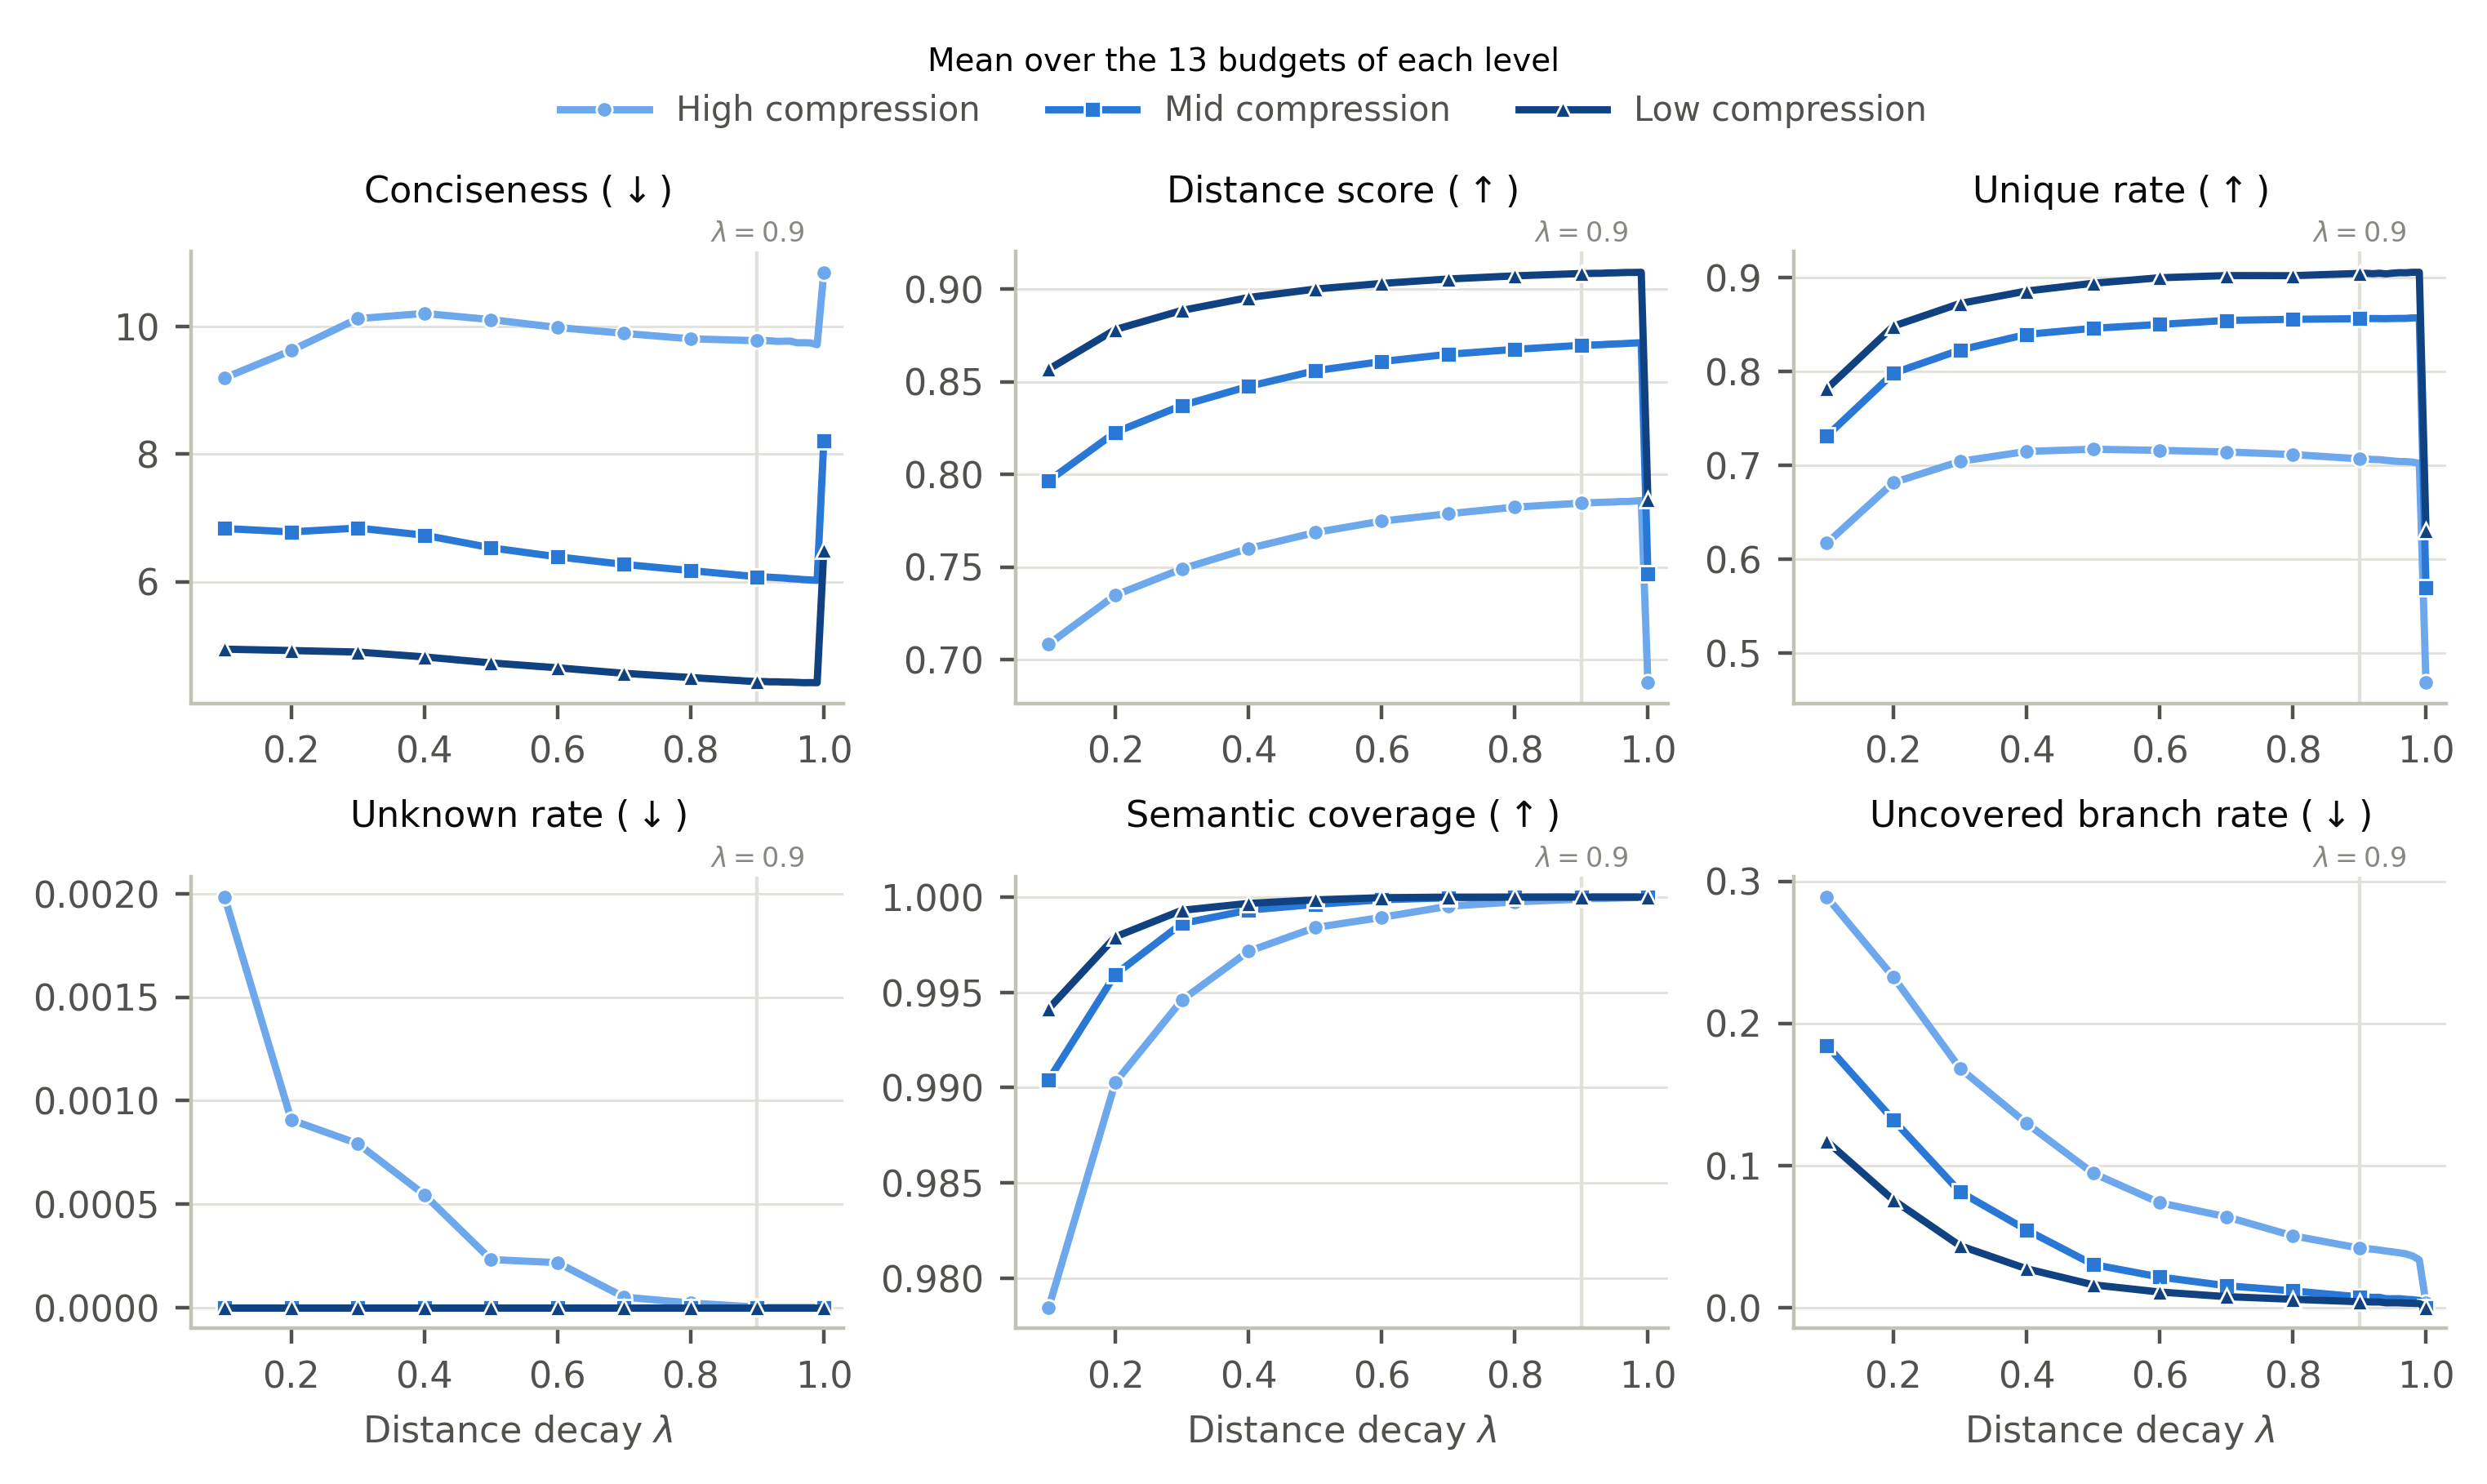
\includegraphics[width=\textwidth]{paper/imgs/metrics_vs_lambda_no0.png}
\caption{Mean metrics of our method as a function of the distance decay $\lambda$, averaged over the 13 token budgets of each compression level.
Lines include $\lambda = 0.91$ to $0.99$; markers show steps of 0.1.
The vertical line marks the default $\lambda = 0.9$.
$\lambda = 0$ is omitted for readability; its values are in Table~\ref{tab:lambda}.}
\label{fig:metrics-vs-lambda}
\end{figure*}

\section{Metrics as a function of \texorpdfstring{$k$}{k}, including random selection}
\label{app:metrics-vs-k-all}

\begin{figure*}[h]
\centering
\includegraphics[width=\textwidth]{paper/imgs/metrics_vs_k_all.png}
\caption{Core metrics as a function of the token budget $k$ for the methods of Figure~\ref{fig:metrics-vs-k}, with random selection (mean over 20 draws) added. Arrows indicate the preferred direction; vertical lines separate the high, mid and low compression levels.}
\label{fig:metrics-vs-k-all}
\end{figure*}

\section{Detailed results on the HERO data}
\label{app:hero}

Table~\ref{tab:ehr} gives the values of Figure~\ref{fig:hero} for every token budget, together with the uncovered branch rate and the share of concepts with a unique representation.
Table~\ref{tab:longtail} details, by frequency bin at $k = 5{,}000$, how much the tokens of each concept borrow events from other concepts.

\begin{table}[t]
\centering
\small
\setlength{\tabcolsep}{3.5pt}
\begin{tabular}{@{}r rr rr r rrr r r@{}}
\toprule
 & \multicolumn{2}{c}{Concepts} & \multicolumn{2}{c}{Events} & Uncov. & \multicolumn{3}{c}{Unique} & Rare, & Tokens \\
\cmidrule(lr){2-3}\cmidrule(lr){4-5}\cmidrule(lr){7-9}
$k$ & Ours & Trunc. & Ours & Trunc. & branch & Tree & Flat & Tree, ev. & tokens $\ge 10$ & per event \\
\midrule
250 & $>$99.9 & 1.5 & $>$99.9 & 82.2 & 25.8 & 51.8 & 41.9 & 21.4 & 100.0 & 9.3 \\
500 & $>$99.9 & 3.1 & $>$99.9 & 92.5 & 16.2 & 56.8 & 50.5 & 29.8 & 100.0 & 8.6 \\
1,000 & 100.0 & 6.1 & 100.0 & 97.5 & 10.3 & 62.3 & 58.7 & 41.2 & 100.0 & 7.6 \\
2,000 & 100.0 & 12.2 & 100.0 & 99.3 & 5.3 & 69.3 & 67.1 & 55.1 & 99.8 & 6.9 \\
3,500 & 100.0 & 21.4 & 100.0 & 99.8 & 2.9 & 75.1 & 73.9 & 65.3 & 97.9 & 6.0 \\
5,000 & 100.0 & 30.5 & 100.0 & 99.9 & 1.5 & 79.1 & 78.2 & 68.0 & 94.1 & 5.6 \\
7,500 & 100.0 & 45.8 & 100.0 & $>$99.9 & 0.7 & 83.9 & 83.5 & 73.3 & 85.7 & 5.2 \\
10,000 & 100.0 & 61.1 & 100.0 & $>$99.9 & 0.3 & 88.5 & 88.1 & 77.8 & 76.1 & 4.8 \\
16,370 & 100.0 & 100.0 & 100.0 & 100.0 & 0.0 & 97.3 & 97.3 & 98.5 & 51.6 & 1.8 \\
\bottomrule
\end{tabular}
\caption{Our tokenizer ($\lambda = 0.9$) and frequency truncation (Trunc.) on the HERO data; all values in \% except tokens per event.
Concepts, Events: share of the 16,370 concepts, and of the 279 million events, represented by at least one token other than the unknown token.
Uncov.\ branch: concepts whose context tree has at least one branch without a token.
Unique: concepts whose representation no other concept shares, with the context tree or with the flat token set, and the same share for the tree counted in events (Tree, ev.); under truncation, the unique shares equal the Concepts and Events columns.
Rare, tokens $\ge 10$: rare concepts (fewer than 100 events) whose every token occurs in at least 10 events.
Truncation costs one token per event; $k = |\Mhero| = 16{,}370$ keeps every concept.}
\label{tab:ehr}
\end{table}

\begin{table}[t]
\centering
\small
\setlength{\tabcolsep}{4pt}
\begin{tabular}{@{}lrrrrr@{}}
\toprule
 & Unique & \multicolumn{4}{c}{Least frequent token} \\
\cmidrule(l){3-6}
Events of the concept & tree (\%) & Events & Gain & $\ge 10$ events (\%) & No gain (\%) \\
\midrule
$< 10$ & 84.3 & 535 & 185.1 & 89.0 & 9.0 \\
$[10, 100)$ & 80.0 & 763 & 25.5 & 100.0 & 8.2 \\
$[100, 1{,}000)$ & 78.0 & 1,759 & 6.3 & 100.0 & 6.7 \\
$\ge 1{,}000$ & 66.5 & 61,017 & 3.6 & 100.0 & 7.0 \\
\bottomrule
\end{tabular}
\caption{Borrowed strength on the HERO data at $k = 5{,}000$, by number of events of the concept; the first two rows are the rare concepts.
Unique tree: concepts whose context tree no other concept shares.
Least frequent token: median number of events of the least frequent token of a concept; median ratio of this number to the concept's own number of events (gain); share of concepts whose least frequent token occurs in at least 10 events; and share with a gain of exactly 1 (no gain).
Under truncation, every kept concept has a gain of 1.}
\label{tab:longtail}
\end{table}

\section{Expert evaluation materials}
\label{app:expert}

Table~\ref{tab:expert-strata} gives the inclusion funnel and the sizes of the strata used to sample and weight the expert ratings (Section~\ref{sec:method:expert}).
\notetoself{add the rater instructions and a screenshot of the form}

\begin{table}[h]
\centering
\small
\setlength{\tabcolsep}{5pt}
\begin{tabular}{@{}llrrr@{}}
\toprule
\multicolumn{5}{@{}l}{\textit{(a) Inclusion funnel}} \\
\multicolumn{4}{@{}l}{Concepts of the HERO data} & 16,370 \\
\multicolumn{4}{@{}l}{\quad in the official SNOMED~CT release (fully defined or primitive)} & 11,796 \\
\multicolumn{4}{@{}l}{\quad\quad whose two context trees differ} & 7,490 \\
\multicolumn{4}{@{}l}{\quad\quad\quad with at most 16 tokens in the two trees together (eligible)} & 3,726 \\
\midrule
\multicolumn{5}{@{}l}{\textit{(b) Strata}} \\
Category & Status & Population & Eligible & Sampled \\
\midrule
Token in ours only & fully defined & 1,200 & 648 & 20 \\
 & primitive & 620 & 558 & 10 \\
Token in the baseline only & fully defined & 272 & 259 & 12 \\
 & primitive & 200 & 200 & 8 \\
Decomposed by both & fully defined & 3,535 & 1,023 & 34 \\
 & primitive & 1,663 & 1,038 & 16 \\
\midrule
Not rated: same tree & & 3,073 & & \\
Not rated: token in both & & 1,233 & & \\
\bottomrule
\end{tabular}
\caption{Expert evaluation: our tokenizer vs Personalized PageRank at $k = 5{,}000$ on the HERO data. Population: concepts of the official release in the stratum, used as weights. Concepts with the same tree, or kept as a token by both methods, count as ``no clear difference''.}
\label{tab:expert-strata}
\end{table}
